\chapter{Vorgehensmodelle zur Softwareentwicklung}
\label{cha:vorgehensmodelle}

%----------------------------------
%
% Klassische Entwicklungsweise am Beispiel des Wasserfallmodells
%
%----------------------------------
    \section{Klassische Entwicklungsweise am Beispiel des Wasserfallmodells}
    \label{sec:wasserfall}

        In diesem Abschnitt wird das Wasserfallmodell als ein Beispiel für eine klassische Herangehensweise der Softwareentwicklung betrachtet. Das Wasserfallmodel ist ein häufig verwendetes Modell in der Softwareentwicklung. Es bildet die Grundlage zu weiteren Verfahren, wie beispielsweise dem V-Modell, das versucht die Tests der Software deutlich früher einzubinden. Im ersten Teil dieses Abschnitts wird dieses vorgestellt und die einzelnen Phasen erläutert und im zweiten Teil werden die gängigen Kritiken am Wasserfallmodell erklärt.

        Dieser Abschnitt dient dazu einen Vergleichswert zu agilen Methoden zu schaffen und, um die Vor- und Nachteile der klassischen Modelle, mit denen der agilen Entwicklungsmethoden, vergleichbar zu machen.

        \subsection{Vorgehensweise des Wasserfallmodels}

        Das Wasserfallmodel gibt eine Menge von Phasen für die Softwareentwicklung vor, bei der jede Phase vollständig abgeschlossen werden muss, bevor die nächste Phase beginnt.

        \begin{figure}[!htbp]
                \begin{center}
                    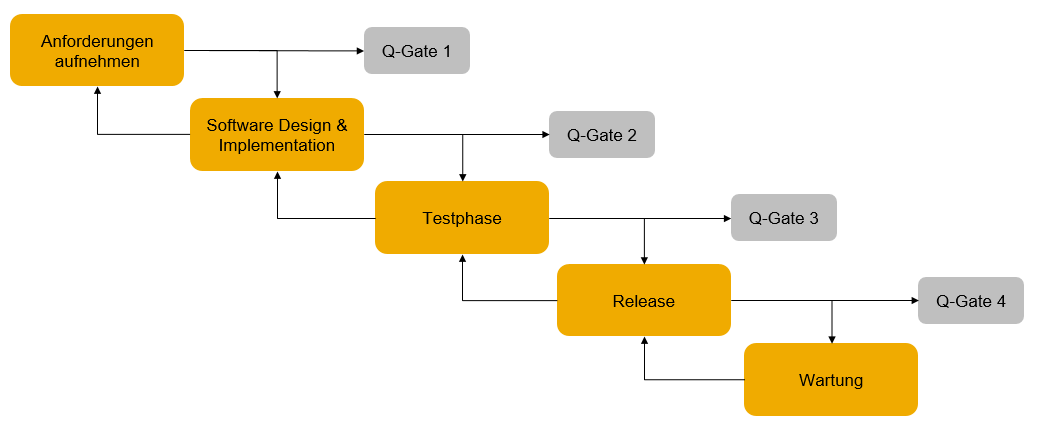
\includegraphics[width=12cm]{Abbildungen/waterfall}
                    \caption[Wasserfallmodell zur Softwareentwicklung]{Wasserfallmodell zur Softwareentwicklung\protect\footnotemark}
                    \label{abb:waterfall}
                \end{center}
        \end{figure}

        \footnotetext{Eigene Abbildung in Anlehnung an Petersen (Waterfall Model).}

        Dies wird in \autoref{abb:waterfall} dargestellt. Die in gold hervorgehobenen Elemente stellen den Hauptprozess einer Variante des Wasserfallmodels dar und die grau markierten Elemente stehen für so genannte \emph{Quality Gates}. Quality Gates stellen häufig eine Checkliste dar, mit deren Hilfe überprüft werden kann, ob alle Schritte der vorhergegangenen Phase absolviert sind.

        In der ersten Phase werden die Anforderungen des Kunden an das Softwareprojekt aufgenommen und formalisiert. Dies umfasst eine umfangreiche Spezifikation, die das Ziel des Projektes konkret vorgibt.\footnote{Vgl. Petersen (Waterfall Model), S.389.}

        Im Anschluss daran wird die Lösung entworfen und implementiert. Dies umfasst eine vollständige Architektur der Software, auf deren Grundlage die Implementation stattfindet. Im Rahmen des Quality Gates wird überprüft, ob in der Design und Implementierungsphase die Anforderungen aus der ersten Phase des Wasserfallmodels erfüllt wurden. Wenn Anforderungen nicht erfüllt sind, muss die Implementierung überprüft werden, oder die Anforderungen müssen überarbeitet werden.\footnote{Vgl. Petersen (Waterfall Model), S.389.}
        Eine Ergänzung des Wasserfallmodels ist die Möglichkeit bei einem neuen Kenntnisstand zu vorherigen Phasen zurückzukehren, um dort nachzubessern.\footnote{Vgl. Royce (Development of large software systems), S.329.}
        Zu diesem Zeitpunkt besteht im Entwicklungsprozess das erste Mal ein lauffähiges Produkt.

        Nach der Implementierung wird die Software erstmals umfangreich getestet. Hierbei sollen alle möglichen Programmabläufe und Konfigurationen geprüft werden.\footnote{Vgl. Petersen (Waterfall Model), S.389.} Eine umfangreichere Betrachtung von Softwaretests folgt in \autoref{cha:einfuehrungQS}.

        Der Release der Software entspricht der Produktivsetzung eben dieser. Ab diesem Moment können Anwender die entwickelte Software verwenden.\footnote{Vgl. Petersen (Waterfall Model), S.390.} Häufig wird der Release mit Schulungen für die Anwender verbunden.

        Den Abschluss bildet die Wartung der Software, falls im Rahmen der produktiven Anwendung weitere Fehler auftauchen.

        \subsection{Probleme und Herausforderungen im Wasserfallmodell}

            Die Testphase der Software im Wasserfallmodell ist für das Projekt häufig sehr kritisch, da sie sehr arbeitsintensiv und zeitaufwändig ist. Werden Fehler gefunden, müssen diese verbessert werden und es entsteht ein iteratives Vorgehen, dass sich abhängig von der Zahl und Komplexität der Fehler sehr lange hinziehen kann.\footnote{Vgl. CTG (Survey of System Development), S.1.}

            Ein weiterer Kritikpunkt am Wasserfallmodell ist, dass erst sehr spät im Projekt eine lauffähige Software entsteht und somit das Projekt zwingend zu Ende geführt werden muss, damit es einen Mehrwert liefern kann.\footnote{Vgl. CTG (Survey of System Development), S.1.}

            Schließlich werden Entscheidungen zu Design, Implementation und Tests sehr früh im Projekt getroffen werden und dies häufig auf einer unzureichenden Faktenbasis.\footnote{Vorwort von Jim Highsmith in Poppendieck (Lean Software Development).} Die Annahmen, die zu Beginn des Projektes getroffen werden lassen sich nur schwer Rückgängig machen, da zu diesen umfangreiche Dokumentationen bestehen, die verändert werden müssen.

%----------------------------------
%
% Prinzipien der agilen Softwareentwicklung
%
%----------------------------------
    \section{Prinzipien der agilen Softwareentwicklung}
    \label{sec:agilePrinzipien}

        \begin{quote}
          \enquote{Achieving a product which satisfies the user's needs normally requires an iterative approach to software development with continual feedback from a user perspective.}\footnote{ISO 9126-1 (Information Technology), S.4.}
        \end{quote}

        Agile Methoden verfolgen das Ziel den Endbenutzer früher in die Softwareentwicklung einzubeziehen, um ein Produkt zu entwerfen, dass tatsächlich benötigt wird. Hierzu werden möglichst schnell und möglichst viele einzelne, aber lauffähige Code-Fragmente entwickelt, die dem Kunden vorgeführt werden um diesen ein Gefühl für die Software zu geben. Das frühe Feedback des Kunden ermöglicht es, bereits während des Entwicklungsprojekts Anpassungen vorzunehmen, um die realen Bedürfnisse zu erfüllen.

        Hierzu existieren Prinzipien, die einfach und granular die Idee der agilen Entwicklung herunterbrechen. Diese werden im agilen Manifest festgehalten und verbreitet.\footnote{Vgl. Beck (Agile Manifesto).}

        \subsection{Individuals and interactions over processes and tools}

            Klassische Softwareentwicklung ist sehr weit standardisiert und geplant. Dadurch sind die Entwickler häufig sehr unflexibel und können nicht auf Wünsche oder Anpassungsvorschläge reagieren, wenn diese den Zeitplan verletzen.\footnote{Vgl. Schneider (Abenteuer Softwarequalität), S.187.}

            Um dieser Entwicklung entgegenzuwirken stellt das agile Manifest die Interaktion mit dem Kunden und den Entwicklern an erste Stelle, anstatt, dass diese von Prozessen regiert werden.

            Insgesammt soll so ein reger Austausch gefördert und auf die Bedürfnisse der einzelnen Personen soll eingegangen werden.\footnote{Vgl. Sutherland, (Agile Softwareentwicklung).}

        \subsection{Working software over comprehensive documentation}

            Durch einen hohen bürokratischen Aufwand und eine umfangreiche Planung der Software wird zu Beginn des Projektes sehr viel Arbeitskraft investiert, ohne, dass diesen ein konkreter Mehrwert gegenüber steht. Durch die dynamische Grundhaltung bei der agilen Entwicklung wird zu Beginn sehr wenig Zeit in die Planung investiert, die Entwicklung wird direkt gestartet und schon nach kurzer Zeit gibt es lauffähige Programmbestandteile.\footnote{Vgl. Sutherland, (Agile Softwareentwicklung).}

            Dieses Prinzip drückt aus, dass der Aufwand der Dokumentation nicht größer sein soll, als der Entwicklungsaufwand. Dem Projektteam soll bewusst sein, dass eine ausführbare Software mehr wert innehat, als eine umfangreiche Planung und Dokumentation einer unfertigen Software.

        \subsection{Customer collaboration over contract negotiation}

            Die SAP SE hat als Hersteller von Standardsoftware zur Unternehmenssteuerung das Ziel Software zu entwickeln und diese zu verkaufen. Der Verkauf von Software wird erheblich erleichtert, wenn diese ein Bedürfnis des Kunden erfüllt und die tägliche Arbeit für diesen erheblich vereinfacht.

            Um die Anforderungen des Kunden zu verstehen und bei der Entwicklung der Software zu berücksichtigen, sollte dieser schon früh einbezogen werden. Die agilen Methoden sollen dabei auf die Wünsche des Kunden reagieren, statt jede Abweichung eines aufgestellten Plans mit umfangreichem bürokratischen Aufwand nachzuverhandeln.\footnote{Vgl. Sutherland, (Agile Softwareentwicklung).}

        \subsection{Responding to change over following a plan}

            Insbesondere bei längeren Projekten ist es meist absurd anzunehmen, dass die Anforderungen des Unternehmens in ferner Zukunft bekannt sind. Bei Unternehmen der Finanzindustrie werden häufig neue regulatorische Anforderungen veröffentlicht oder das Marktumfeld verändert sich. Um auf diese Änderungen auch während der Projektlaufzeit eingehen zu können und keine zum Release veraltete Software einzusetzen sollte im Projekt auf Veränderungen eingegangen werden.\footnote{Vgl. Sutherland, (Agile Softwareentwicklung).}

%----------------------------------
%
% Ausgewählte Methoden der agilen Softwareentwicklung
%
%----------------------------------
    \section{Ausgewählte Methoden der agilen Softwareentwicklung}
    \label{sec:agileMethoden}

        Im Folgenden werden konkrete Herangehensweisen zur agilen Entwicklung vorgestellt. Diese sind genau wie die Prinzipien des agilen Manifests sehr allgemein und flexibel gehalten, um den Entwicklern hinreichend Freiraum zu geben um Ideen ausleben zu können.

        \subsection{Lean Software Development}

            Die Grundlage des Lean Software Developments bildet der Produktentwicklungsprozess von Toyota. Im Anschluss an den zweiten Weltkrieg wurde dort die Automobilproduktion aufgebaut und da in Japan weder der Platz noch die Ressourcen vorhanden waren, um die ineffiziente amerikanische Automobilproduktion zu immitieren, wurden neue Prinzipien in die Entwicklung integriert, die die Lagerhaltung, Massenfertigung und Produktentwicklung betreffen.\footnote{Vgl. Dombrowski (Lean Development), S.7.}

            Die bisherige Annahme im Produktentwicklungsprozess, unabhängig von Software, Autos o.ä., war, dass ein Fehler, der während der Planung eliminiert wird um den Faktor 1000 günstiger ist als ein Fehler, der beim Kunden entdeckt wird. Dies leitet sich aus der so genannten Zehnerregel der Fehlerkosten ab. \autoref{abb:zehnerregel} illustriert die exponentiell wachsenden Fehlerkosten. Ein Fehler, der einen Euro kostet, wenn er während der Planung entdeckt wird, kostet, wenn er beim Kunden entdeckt wird, beispielsweise 1000 Euro. Das Modell der Zehnerregel sagt aus, dass Fehler, die durch eine umfassende Fehlerprävention früh gefunden werden, trotz erhöhter Qualitätssicherungskosten, in der Summe günstiger sind, als Fehler, die erst sehr spät entdeckt und nachträglich ausgebessert werden müssen.\footnote{Vgl. Brüggemann (Grundlagen Qualitätsmanagement), S.29.}

            \begin{figure}[!htbp]
                \begin{center}
                    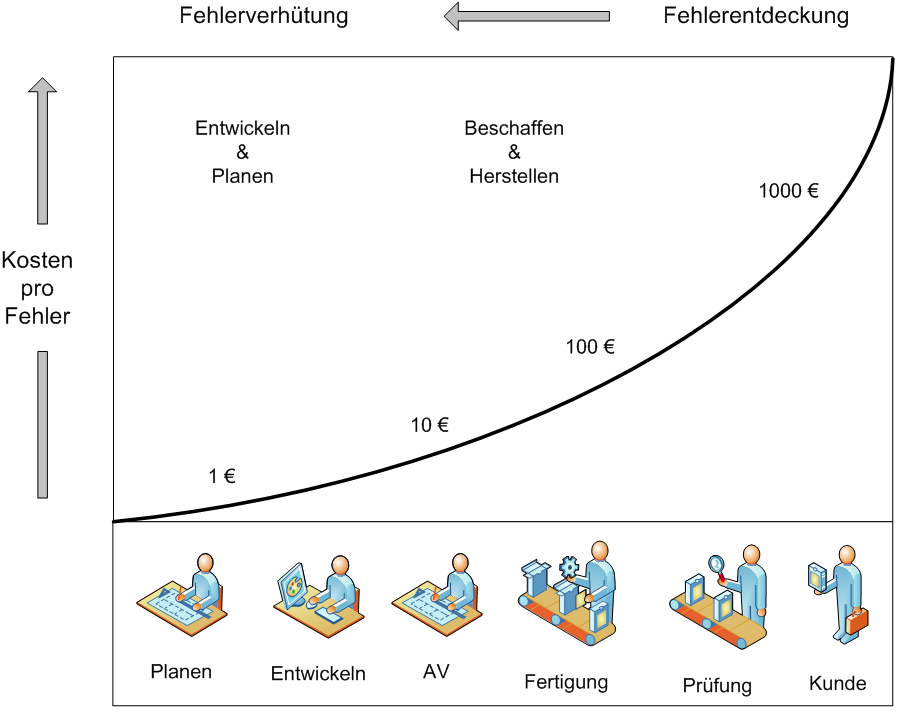
\includegraphics[width=11cm]{Abbildungen/zehnerregel}
                    \caption[Zehnerregel der Fehlerkosten]{Zehnerregel der Fehlerkosten\protect\footnotemark}
                    \label{abb:zehnerregel}
                \end{center}
            \end{figure}

            \footnotetext{Six Sigma Black Belt (Zehnerregel der Fehlerkosten).}

            Im Rahmen von Lean Development halten sich die praktizierenden Unternehmen während des Designprozesses jedoch möglichst viele Optionen offen, um während des Produktionsprozesses Entscheidungen auf einer optimalen Faktenbasis zu treffen und nicht auf Basis plausibler Annahmen.\footnote{Vgl. Poppendieck, 2003, S.5.} Solche Design- und Funktionsentscheidungen werden in agilen Methoden erst sehr spät getroffen, da die Anforderungen des Kunden erst zu Beginn jeder Iteration festgelegt werden und nicht in einem umfangreichen Scopedokument zu Beginn des gesamten Projektes.

             Einige Prinzipien des Lean Developments lassen sich zwar auf klassische Softwareentwicklungsmethoden anwenden, sind aber in einem agilen Umfeld leichter zu praktizieren und implementieren. Der Entwicklungsprozess baut auf sieben Prinzipien auf, die zusammen mit agilen Methoden auch auf die Softwareentwicklung angewendet werden können.\footnote{Vgl. Poppendieck (Lean Software Development), S.13.}:

            \begin{itemize}
                \item Eliminiere Überschuss
                \item Verstärke Lernprozesse
                \item Triff Entschiedungen so spät wie möglich
                \item Liefer Endprodukte so schnell wie möglich
                \item Stärke das Team
                \item Fördere Integrität
                \item Hab eine allumfassende Perspektive
            \end{itemize}

            Im Folgenden wird eine kurze Einführung der Prinzipien gegeben, mit einer Erläuterung, wie sie als agiler Prozess aufzusetzen sind.

            \enquote{Waste is anything that does not add value to a product, value as perceived by the customer.}\footnote{Poppendieck (Lean Software Development), S.13.} Der Überschuss umfasst, bezogen auf die Softwareentwicklung, nicht nur sämtliche Applikationen, die nicht benötigt werden. Vielmehr enthält er auch ungenutzte Funktionen, sowie das Potenzial zu möglichen, zukünftigen Erweiterungen im Programm. Das Ziel sollte es sein, den Umfang des Programms so klein wie möglich zu halten, um die unmittelbaren Bedürfnisse des Kunden zu befriedigen. Das bedeutet, dass in jeder Iteration des Entwicklungsprozesses nur die Funktion entwickelt wird, die der Anwender braucht und die am höchsten priorisiert ist. Rein statistisch werden etwa 50\% aller Funktionen einer Software selten oder nie genutzt.\footnote{Ebert (Software Measurement).} Wenn dieser Überschuss eliminiert wird, werden die Programme schlanker, einfacher und günstiger in der Wartung, ohne das der Anwender auf wichtige Funktionen verzichten muss.

            Die Entwicklung eines Produktes ist im Gegensatz zur Herstellung eines Produktes kein linearer Prozess, der vorher skizziert und abgearbeitet werden kann. Obwohl die Variation in der Produktion reduziert, beziehungsweise eliminiert werden soll, ist sie im Entstehungsprozess eines Produkts durchaus wünschenswert, um die bestmögliche Lösung zu finden.\footnote{Vgl. Ballard (Iteration in design), S. 2f.} Damit möglichst viele Optionen betrachtet werden, und, um sich mit fortgeschrittenem Kenntnisstand für eine zu entscheiden hat Toyota das so genannte \emph{Set-Based Concurrent Engineering} entwickelt. Hierbei werden mehrere Prototypen in die Entwicklung mitgeführt, statt direkt zu Entwicklungsbeginn einen Designstop einzulegen. Diese Protoypen werden mit dem jeweils aktuellen Kenntnisstand weiterentwickelt und eine Entscheidung zu Gunsten einer Variante fällt so spät wie möglich. Zur Entwicklung dieser Methoden wird ein Prozess von drei Oberpunkten vorgesehen, die die Menge von Möglichkeiten filtern:

            \begin{itemize}
                \item \enquote{Map the design space
                \item Integrate by intersection
                \item Establish feasibility before commitment}\footnote{Sobek (Set-Based Concurrent Engineering), S.73.}
            \end{itemize}

            Zunächst wird daher der Rahmen festgelegt, in dem entwickelt werden darf. Dies betrifft, übertragen auf die Softwareentwicklung, Programmiersprachen und Systeme. Im Anschluss werden Konzepte in diesem Rahmen übereinandergelegt und die Variation auf das Nötigste reduziert. Abschließend werden alle verbliebenen Vorgehensweisen auf Machbarkeit geprüft und auf Basis dieses Ergebnisses wird eine Entscheidung getroffen. Bis zur Entscheidung für eine Vorgehensweise lernen die Entwickler aus dem Entwicklungsprozess. Schließlich wird die Möglichkeit, die den größten Nutzen bietet umgesetzt. Dies ist auch der Grund dafür, dass eine möglichst späte Entscheidung angestrebt wird.\footnote{Vgl. Sobek (Set-Based Concurrent Engineering), S.73f.}

            Die Vorgabe so schnell wie möglich Ergebnisse zu liefern bedeutet nicht, dass ein unfertiges oder unreifes Produkt ausgeliefert werden soll, sondern, dass lauffähige Versionen entstehen, auf deren Grundlage die Entwicklung voranschreiten kann. Somit kann ein Kunde herausfinden, was er benötigt und die Richtung des Projektes besser gesteuert werden. Dies führt zu kurzen Iterationen, die lauffähige Ergebnisse liefern.\footnote{Vgl. Poppendieck (Lean Software Development), S.74ff.}

            Die reine Anwendung von Prozessen führt häufig nicht zu den gewünschten Ergebnissen. Vielmehr geht es ebenfalls darum, die Mitarbeiter in den Prozess der Produktentstehung einzubinden und somit alle Ideen und Kompetenzen zu nutzen. Bisherige Softwareentwicklungsprozesse zielen darauf ab, zu Beginn der Entwicklung Entscheidungen von einer Hand voll Personen treffen zu lassen, die die tatsächliche Implementierung meist nicht persönlich umsetzen. In einem Lean Development Umfeld sollen die Entscheidungen von den umsetzenden Personen getroffen werden und die oberen Hierarchien durch Reports, Grafiken und regelmäßige Meetings lediglich informiert werden. Dies beschleunigt Iterationen und ermöglicht mehr Tests und Versuche, die zu besseren Ergebnissen führen.\footnote{Vgl. Poppendieck (Lean Software Development), S.98ff.}

            Die Integrität einer Software wird daran gemessen, wie zufrieden jemand ist, der mit dieser Software arbeitet, unabhängig davon, ob eben dieser Anwender oder Entwickler ist. Hierbei beruft sich Poppendieck auf die Qualitätskriterien von Software der ISO 9126-1, die oben vorgestellt werden. Sie sagt, dass diese Kriterien nicht durch Prozesse und Messungen umsetzbar sei, sondern durch weise Führung, fachliche Expertise, effiziente Kommunikation und gesunde Disziplin.\footnote{Vgl. Poppendieck (Lean Software Development), S.123ff.} Der Weg zur Integrität einer Software basiert daher auch auf einigen Prinzipien des agilen Manifests.

            Zuletzt soll das Gesamtziel des Projektes nicht aus den Augen verloren werden. Die absolute Optimierung eines Teilbereichs zu Lasten des Gesamtprojekts sollte zwingend vermieden werden.\footnote{Vgl. Poppendieck (Lean Software Development), S.146f.}

            Zusammenfassend ist Lean Software Development eine Menge von Prinzipien, die aus der Entwicklung von Autos abgeleitet wurde und zu Beginn eines Projektes als konkrete Pläne umgesetzt werden sollen. Wie die im Folgenden vorgestellten agilen Programme weißt es auf typische Fehler hin und gibt Ratschläge, wie sie vermieden werden können, ohne hierbei die Freiheit des Teams einzuschränken.

        \subsection{Extreme Programming}

            \begin{quote}
                \enquote{XP is a style of software development focusing on excellent application of programming techniques, clear communication, and teamwork which allows us to accomplish things we previously could not even imagine.}\footnote{Andres (Extreme Programming).}
            \end{quote}

            Extreme Programming räumt mit einigen Konventionen der Softwareentwicklung auf, indem es die bisher bestehenden Prozesse bewusst kritisiert und eigene Werte und Modelle präsentiert, die die Softwareentwicklung vereinfachen. Es legt einen Prozess fest, der die Kommunikation und Kollaboration im Team fördert und Prozessteile der Softwareentwicklung überspitzt anwendet. So werden beispielsweise die Tests nicht im nachhinein durchgeführt, sondern vor der Entwicklung der Software entwickelt und automatisiert, sodass nach jeder Veränderung der Software die korrekte Funktionalität überprüft werden kann.

            \begin{figure}[H]%[!htbp]
                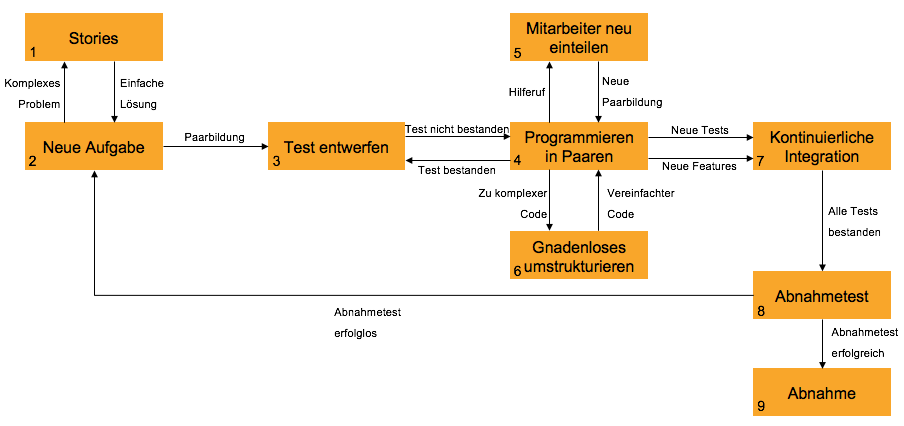
\includegraphics[width=15cm]{Abbildungen/XP_vorgehensmodell}
                \caption[Vorgehensmodell des Extreme Programming]{Vorgehensmodell des Extreme Programming\protect\footnotemark}
                \label{abb:xpmodel}
            \end{figure}

            \footnotetext{Eigene Abbildung in Anlehnung an Uni Saarland (Extreme Programming).}

            \autoref{abb:xpmodel} zeigt das Vorgehensmodell des Extreme Programming, dessen Bestandteile im Anschluss genauer erläutert werden. Das Vorgehen beginnt mit einer neuen Aufgabe (Element 2 der Abbildung), die in das Team übergeben wird und durch User Stories vereinfacht wird, bis sie in den Kreislauf übergeben werden kann. Nach der Fertigstellung einer Aufgabe wird mit einer neuen Aufgabe begonnen, bis alle Aufgaben des Programms abgenommen wurden.

            Extreme Programming orientiert sich dennoch an einem groben Prozess zur Entwicklung von Software. Zunächst wird eine User Story entworfen (Element 1), das heißt ein Anwender beschreibt was er tun muss und an welchen Stellen er dabei unterstützt werden muss.\footnote{Vgl. Uni Saarland (Extreme Programming).} Zur Erläuterung des Prozesses wird nachfolgend beispielhaft das Anlegen eines Vertrags in einer Filiale aus Sicht eines Angestellten betrachtet.

            Der Anwender möchte die Daten des Kunden in die Softwareoberfläche eintragen und anschließend einen Vertrag mit den Konditionen für diesen Kunden ausdrucken. Die Daten sollen zudem in der Datenbank der Bausparkasse hinterlegt werden. Daraus ergibt sich eine neue Aufgabe für die Softwareentwickler.

            Extreme Programming sieht vor, dass für jede zu entwickelnde Komponente zunächst ein Test (Element 3) geschrieben wird. Die Tests bilden das Pendant zur klassischen Spezifikation und werden nach jeder Änderung der Software überprüft, um so eine ständige Lauffähigkeit des Moduls zu gewährleisten. Ein Test würde beispielsweise prüfen, wie mit unvollständigen Angaben umgegangen wird oder wie verfahren wird, wenn kein Drucker erreichbar ist. Bei der Erstellung der Test-Fälle sollen alle gewöhnlichen Eingaben, ungültige Eingaben und Randwerte geprüft werden.\footnote{Vgl. Wells (Unit Tests).}

            Auf Grundlage der entworfenen Tests startet die Entwicklung, die die Ansprüche des Anwenders, die im Test formalisiert wurden, erfüllen soll. Im Gegensatz zur klassischen Entwicklung von Software, bei der jeder Entwickler für einen Baustein des Programms zuständig ist und diesen in Einzelarbeit vorantreibt, wird im Extreme Programming Pairprogramming empfohlen (Element 4). Dies bedeutet, dass zwei Programmierer zur gleichen Zeit am selben Computer arbeiten und eine Person tippt, während die andere Person die Entwicklung kontrolliert. Außerdem sollen alle Entwickler jederzeit den gesamten Code kennen und dürfen an jeder Stelle etwas verändern, sobald sie Fehler entdecken. Das Ziel ist es die Abhängigkeit von einzelnen Entwicklern zu reduzieren und schon während der Entwicklung eine ständige Kontrolle durch den Partner zu haben. Studien haben außerdem nachgewiesen, dass zwei Entwickler die Entwicklungszeit reduzieren und weniger Fehler produzieren.\footnote{Williams (Pair-Programming), S.5f.}

            Extreme Programming hat darüber hinaus noch zwei Prinzipien, die bei der klassischen Softwareentwicklung in dieser Form nicht angewendet werden. Zunächst wird immer nur ein aktuelles Problem gelöst und es werden keine Pläne für zukünftige Integrationen und Erweiterungen im Code umgesetzt. Der Code soll so einfach wie möglich gehalten werden. Die Idee dahinter ist, dass ein einfacher Code besser anzupassen ist, als komplizierter Code mit einer Schnittstelle, die eventuell nie gebraucht wird.\footnote{Rumpe (Extreme Programming), S.3.}

            Das zweite Prinzip ist der selbstdokumentierende Code. Über sprechende Methodennamen und Kommentare soll jeder Entwickler zu jeder Zeit verstehen, was sich der Autor des Codes gedacht hat. Sprechender Code soll die Dokumentation der Software obsolet machen. Dies geschieht aus dem Grund, dass Dokumentationen häufig nicht aktuell sind oder nicht mit dem gleichen Eifer wie der Code entwickelt werden und somit fachlich falsch sind. Diese Ziele werden erreicht, indem sehr viele Kommentare verwendet werden und das bisher entwickelte \emph{Refactored} wird. Das bedeutet, dass Codebruchstücke, wie beispielsweise eine Tabellenabfrage in eine Methode ausgegliedert werden und stattdessen die Methode im Hauptprogramm aufgerufen wird. Diese ständigen Restrukturierungen vereinfachen das bisher Entwickelte und lassen den Umfang des Programms nicht ausufern.\footnote{Rumpe (Extreme Programming), S.6f.}

            Die entwickelten Bausteine werden meist täglich in die bestehende Software integriert und fortlaufend getestet (Element 7 und 8). Am Ende des agilen Projektes steht die Abnahme (Element 9) durch den Kunden.

            Natürlich stößt auch das Extreme Programming in Projekten an seine Grenzen. Die Pairprogramming Methodiken setzen voraus, dass die Entwickler auf engem Raum zusammenarbeiten, da Pair-Programming Aktivitäten sonst erschwert werden. Außerdem sollte für die häufige Abstimmung und Kommunikation das Team sehr klein gehalten werden, meist werden 9-12 Personen empfohlen.\footnote{Vgl. Uni Saarland (Extreme Programming).}

            Extreme Programming stellt konkrete Anforderungen an das Team und lässt in der Umsetzung die wenigsten Freiheiten der agilen Methoden. Es ist, wie der Name impliziert, eine sehr extreme Herangehensweise, die Tests, Entwicklung und Flexibilität maximiert. Es können jedoch vereinzelte Methoden des Extreme Programming in anderen agilen Verfahren verwendet werden, um einen Teil der methodischen Flexibilität zu erhalten.

        \subsection{Scrum}
        \label{subsec:scrum}

            Scrum ist ein \enquote{Ein Rahmenwerk, innerhalb dessen Menschen komplexe adaptive Aufgabenstellungen angehen können, und durch das sie in die Lage versetzt werden, produktiv und kreativ Produkte mit dem höchstmöglichen Wert auszuliefern.}\footnote{Schwaber (Scrum Guide), S.3.} Es ist
            \begin{itemize}
                \item \enquote{Leichtgewichtig
                \item Einfach zu verstehen
                \item Schwierig zu meistern.}\footnote{Schwaber (Scrum Guide), S.3.}
            \end{itemize}

            Im Gegensatz zum Extreme Programming ist Scrum ein Rahmenwerk statt einer Methode, das neben konkreten Managementvorgaben sehr viel Gestaltungsfreiraum bietet. Scrum setzt auf einen iterativen, inkrementellen Ansatz. Das bedeutet, dass kurze Phasen der Entwicklung ständig wiederholt werden und das Endprodukt Stück für Stück aufgebaut wird. Mit jeder abgeschlossenen Phase wird die Software um einen weiteren Baustein ergänzt.

            Für Scrum-Teams wird eine Personenanzahl von 5-9 Entwicklern zuzüglich Scrum Master und Product Owner empfohlen. Somit soll die Organisation flexibel genug sein, um sich selbst koordinieren zu können, aber groß genug um alle notwendigen Kenntnisse abzudecken, sodass das Team während der Softwareentwicklung nicht auf externe Hilfe angewiesen ist.\footnote{Vgl. Schwaber (Scrum Guide), S.6.} In \autoref{tbl:scrumrollen} werden die Rollen im Scrum-Team zusammengefasst und im Anschluss werden diese erklärt.

            \begin{table}[!htbp]
            \begin{tabularx}{\textwidth}{|l|c|X|}
                \hline
                Name & Anzahl & Aufgaben \\
                \hline
                Product Owner & 1 & Kommunkation mit Kunden \\
                && Verwalten des Product Backlog \\
                && Verantwortung zum Erfolg des Projektes \\
                &&\\
                Scrum Master & 1 & Vermittler zwischen Product Owner und Team \\
                && Erfahrener Ansprechpartner für Fragen zu Scrum \\
                && \\
                Entwickler & 5-9 & Entwicklung der Inkremente \\
                && Einschätzung zu Aufwänden für Sprints \\
                \hline
            \end{tabularx}
            \caption{Rollen im Scrum-Team}
            \label{tbl:scrumrollen}
            \end{table}

            Der Product Owner hat die Verantwortung, dass der Kunde das erhält, was er sich wünscht. Er steht in ständigem Austausch mit diesem, präsentiert Zwischenergebnisse und trägt die neuen Wünsche priorisiert in das Entwicklungsteam. Alle Wünsche und Anforderungen, die an das Team gestellt werden, haben über den Product Owner zu laufen.\footnote{Vgl. Maximini (Scrum), S.167f.}

            Der Scrum Master vertritt die Interessen der Entwickler gegenüber Außenstehenden und dem Product Owner. Er sorgt dafür, dass die Scrum-Regeln eingehalten werden und die Entwickler während ihrer Entwicklungsphasen nicht gestört werden. Der Scrum Master verfügt über keine Weisungsbefugnis, sondern versucht einem Ombudsmann ähnlich Win-Win Situationen für alle Parteien zu erreichen. Als erfahrenes Scrum-Teammitglied steht er außerdem für alle Fragen zur Verfügung und schult seine Kollegen bei Bedarf.\footnote{Vgl. Maximini (Scrum), S.170f.}

            Das Entwicklungsteam setzt sich aus einer Vielzahl von Experten zusammen, die alle benötigten Kompetenzen abdecken. Das gesamte Entwicklungsteam ist verantwortlich für den kompletten Code und organisiert sich vollständig selber.\footnote{Vgl. Schwaber (Scrum Guide), S.5f.}

            Neben dem Team umfasst Scrum auch Vorgaben zum Ablauf. Hierfür werden eine Menge von Meetings und Phasen vorgegeben, die einen festen Zeitraum haben, der nicht überschritten werden darf. Auf Grundlage dieser Annahmen sind Scrum-Projekte sehr planbar.

            \enquote{Das Herz von Scrum ist der Sprint, eine Time Box von maximal einem Monat, innerhalb dessen ein fertiges (\emph{Done}), nutzbares und potenziell auslieferbares Produkt-Inkrement hergestellt wird}\footnote{Vgl. Schwaber (Scrum Guide), S.8.}. Dies entspricht der oben bereits vorgestellten Entstehung von Software durch Bausteine, die ein Grundkonstrukt, um Funktionen erweitern. Wichtig ist dabei, dass jeder Baustein fertig ist, was durch den Ausdruck Done im obigen Zitat versinnbildlicht wird. Die Definition of Done muss von Product Owner, Scrum-Team und Kunde vorab festgelegt und festgehalten werden, damit es dort zu keinen Missverständnissen kommt.

            Ein Sprint dauert für gewöhnlich vier Wochen und beinhaltet eine Menge von Ereignissen:
            \begin{itemize}
                \item Sprint Planning
                \item Daily Scrums
                \item Sprint Review
                \item Sprint Retrospektive
            \end{itemize}

            \begin{figure}[!htbp]
                \begin{center}
                    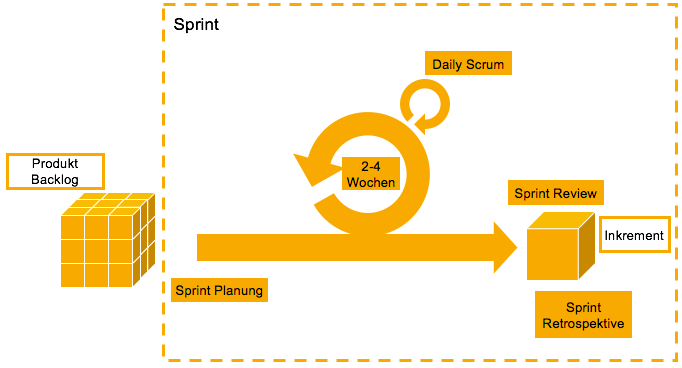
\includegraphics[width=\textwidth]{Abbildungen/scrum}
                    \caption[Planungszyklus Scrum]{Planungszyklus Scrum}
                    \label{abb:scrum}
                \end{center}
            \end{figure}

            \autoref{abb:scrum} illustriert den gesamten Scrum-Ablauf. Alle Einträge des Product-Backlogs werden priorisiert in das Scrum-Team getragen und beim Sprint-Planning werden die die Elemente des Product-Backlogs festgelegt, die in diesem Sprint erledigt werden sollen. Daraus entsteht der Sprint-Backlog. Diese Aufgaben sollen in Phasen von zwei bis vier Wochen abgearbeitet werden. Während des Sprints finden tägliche Meetings statt, die Daily Scrums, die in der Abbildung auf dem Sprintzyklus aufsetzen. Diese klären den Status des Sprints und fördern die Kommunikation im Team. Am Ende des Zyklus steht ein Produktbaustein, das so genannte Inkrement, dass die Software ergänzt und erweitert. Nach dem formalen Abschluss durch Retrospektive und Review wird der Zyklus ausgehend vom Product-Backlog neu begonnen.

            Während des Sprints werden keine weiteren Themen zum Scope ergänzt und weder Zeit- noch Qualitätsplanung angepasst. Erst die Sprint-Planung am Ende jedes Zyklus bietet die Möglichkeit zur Nachkalibrierung. Die Dauer eines Sprints ist daher so gewählt, dass das Projekt flexibel genug ist, um auf Anforderungen einzugehen, aber die Entwickler die Chance erhalten sich voll und ganz auf eine Aufgabe zu konzentrieren und nicht ständig durch Anforderungsänderungen aus ihrem Fokus gerissen werden.\footnote{Maximini (Scrum), S.181f.} Im Folgenden werden die vier Phasen eines Sprints weiter aufgeschlüsselt:

            Das \emph{Sprint Planning} dient als Vorbereitung für den kommenden Sprint. Im Zentrum des Planungsprozesses stehen zwei Fragen, die am Ende des Meetings beantwortet sein sollen.
            \begin{itemize}
                \item Was kann in diesem Sprint fertiggestellt werden?
                \item Wie wird die ausgewählte Arbeit erledigt?
            \end{itemize}

            In der ersten Phase präsentiert der Product Owner die Wünsche des Kunden und priorisiert alle Dinge, die bis zum Ende des Sprints geschafft werden sollen. Das Entwicklungsteam diskutiert mit ihm daraufhin, ob die Zeitplanung und Deadlines realistisch sind. Haben sich Product Owner und Scrum Team auf einen Scope geeinigt, kommt es zu Phase zwei des Sprint Planning, in der geplant wird, wie das Sprint-Ziel zu erreichen ist.\footnote{Vgl. Maximini (Scrum), S.182f.}

            Die Vorgehensweise basiert bei Software grob auf der Codestruktur der Methoden, Eigenschaften von Klassen usw. Sie lässt sich beispielsweise durch \emph{Unified Modelling Language} (UML) Klassendiagramme sehr gut erfassen. Hierbei sollen unabhängig von Kompetenzen und Erfahrungen alle Ideen des Teams eingebracht werden. Ein großes Problem bei Sprint Plannings sind häufig Externe, insbesondere Vorgesetzte, die bei jungen Entwicklerteams oft Ratschläge geben, die aber als Weisung aufgenommen werden. Durch die Präsenz weisungsbefugter Personen wird die Kreativität im Team so häufig untergraben und nicht vollkommen ausgeschöpft.
            Der Scrum Master hat zusätzlich noch die Aufgabe sehr dominante und aktive Personen zu bremsen und auch die ruhigeren Charaktere in die Diskussion mit einzubinden. Während des Sprint Plannings und auch dem gesamten Sprint fungiert er als Moderator.\footnote{Vgl. Maximini (Scrum), S.182f.}

            Das \emph{Daily Scrum} findet täglich statt, dauert meist 15 Minuten und ist ein Meeting mit dem gesamten Team. Um Dynamik zu erzeugen und nicht zu überziehen findet es meist im Stehen, kurz vor der Mittagspause, statt. Das Daily Scrum dient dazu, dem gesamten Entwicklungsteam eine Übersicht zu geben, wer wo steht und wie weit man als Team bei der Verwirklichung des Sprint Ziels ist. Außerdem findet man häufiger eine Lösung, wenn Probleme auftreten und diese im Team vorgestellt werden. Jedes Mitglied des Scrum-Teams ist nacheinander an der Reihe und beantwortet in der großen Runde folgende drei Fragen:

            \begin{itemize}
                \item Was habe ich gestern getan?
                \item Was werde ich bis morgen tun?
                \item Wo bin ich dabei auf Hindernisse gestoßen?
            \end{itemize}

            Insbesondere bei der letzten Frage geht es nicht darum Lösungen während des Daily Scrums zu finden, sondern im Scrum das Problem vorzustellen und jemanden zu finden, der es im Anschluss gemeinsam mit angeht. Somit schweift das Team gedanklich nicht ab, wenn es technischer wird. Dem Daily Scrum kommt somit eine Planungs- und Kontrollfunktion zu \footnote{Vgl. Maximini (Scrum), S.183.}.

            Der \emph{Sprint Review} schließt sich an einen Sprint an, um auf Grundlage der Ergebnisse erneut zu planen. Beim Sprint Review sind neben dem gesamten Scrum-Team auch Stakeholder anwesend, denen das Produkt vorgestellt werden soll. Dabei ist wünschenswert, dass die Stakeholder das Produkt selber testen können und die Entwickler dabei die Wünsche und Gedanken der Stakeholder zum Produkt notieren. Auf Grundlage dieses Feedbacks wird anschließend das Produkt kontrolliert und, falls nötig, der Backlog erweitert.\footnote{Vgl. Maximini (Scrum), S.183.}

            Auf Grundlage der Definition of Done werden im Sprint Review die Backlogeinträge abgehakt, die erfüllt sind und die bestehenden Einträge auf Zeit und Erreichbarkeit überprüft. Das Sprint Review stellt somit die Grundlage zum kommenden Sprint Planning dar.\footnote{Vgl. Schwaber (Scrum Guide), S.16.}

            Die \emph{Sprint Retrospektive} stellt das Pendant zum Sprint Planning dar und schließt einen Sprint formell ab. Während beim Sprint Review das erstellte Produkt im Mittelpunkt steht, betrachtet die Sprint Retrospektive die Zusammenarbeit des Scrum Teams und dessen Arbeitsweise. Das Ziel dieses Meetings ist es, Maßnahmen herauszuarbeiten, die die Zusammenarbeit im Team verbessern oder die die Qualität der Endprodukte verbessern. Am Ende des Meetings soll eine Liste mit wenigen, aber greifbaren Maßnahmen stehen, die jedes Teammitglied bis zum Ende des folgenden Sprints umsetzen kann.\footnote{Vgl. Schwaber (Scrum Guide), S.13.}

            Scrum ist eines der bekanntesten agilen Verfahren und wird häufig als Synonym für eine agile Vorgehensweise genutzt. Es gibt Vorgaben zum Management von Anforderungen und lässt dem Entwicklerteam freien Spielraum zur Umsetzung eben dieser. Scrum-Teams bemühen sich, aus jedem Sprint etwas zu lernen und ihre Vorgehensweise im nächsten Sprint anzupassen, um sich kontinuierlich zu verbessern. 